\chapter{Double Higgs Bosons Analysis}
\label{chap:DoubleHiggs}

\chapterquote{Two is better than one}%
{Sir Steve Orange, 1785--1854}%: Blackwood's Magazine May 1830

\section{Motivation}

Ha there is a higgs.

We found higgs. Higgs is cool. It explains mass.

Why double higgs. Double higgs coulpling is unique to linear collider. It can revel much about the BSM models.

Generator level study has performed. ILC has done this this and that. gHHH in CLIC before

Here we do things differently. First subchannels, then extract both couplings simultaneously.

\section{Theory}

general higgs field

Lagrangian

current constraunt

single higgs coupling measurement done in higgs

Double higgs measurement

The main mechanism for double Higgs production %in \epem collisions
%at high energy CLIC ($\sqrt{s}>$\SI{1}{\TeV}) is via $WW$-fusion ($\epem\to HH\nu\overline{\nu}$). The main Feynman diagrams contributing to the process are illustrated in Figure . %The cross section for the process increases with the centre-of-mass energy: from \SI{0.15}{\fb} at $\sqrt{s}=$\SI{1.4}{\TeV} to \SI{0.59}{\fb} at $\sqrt{s}=$\SI{3}{\TeV}, assuming a %Higgs mass of \SI{126}{GeV}.

\section{Analysis Straggly Overview}

Proof-of-principle study was perform at \CLIC using \CLICILD detector model for \rootS{1.4} and 3\,TeV. Simulated samples, including those containing double higgs production were used. Signal events, events with double higgs production, were selected via a set of carefully designed and complicated methods. \gHHH and \gWWHH are extracted simultaneously with template fitting with modified couplings samples.
\section{Monte Carlo Sample Generation}


% TODO
% Understand bremsstrahlung and EPA
Single channel is defined as \eeToHH. It is divided into sub-channel \eeToHHbbWW and \eeToHHbbbb to allow closer examination and an improvement of signal selection when combined. In particular, I studied \eeToHHbbWW sub-channel.

Selected background samples, including processes initiated by photons, are considered in the analysis and listed in Table \ref{tab:doubleHiggsMCSamples}. These background were expected share similar topologies with the signal process. When describing a multi-quark final state, it is referring to  all final states of the same number of quarks, including final states with possible additional neutrinos and or leptons. A multi-quark final state does not include higgs production, unless explicitly stated.

The usual two-quark and four-quark final states were considered.
Since the significant presence of beamstrahlung, where photon produced due to the high electric field generated by the colliding beams, processes initiated by photons are also included.

Processes invloving real photons from beamstrahlung (BS) and ``quasi-real'' photons are generated separately. For the ``quasi-real'' photon initiated processes, the Equivalent Photon Appproximation (EPA) has been used.

Photon-electron/photon-photon interactions with four-quark final states were considered. Photon-electron interaction with two-quark final state, one Higgs, and one neutrino is considered. Photon-electron interaction with two-quark final state, one Higgs, and one lepton is not considered due to its negligible cross section.

%I have just checked the ea->qqHl and ea->qqHv processes at 3 TeV. While ea->qqHl has a very small cross section (0.07 fb with photon from EPA, 0.6 fb with photon from BS), the ea->qqHv final state might not be negligible (4 fb with photon from EPA, 59 fb with photon from BS). The events will be very forward (more than the signal I assume). But of course I'm producing MC samples so that we can check.

Single higgs productions are not considered because topologies are very different to the single process.
Six-quark final states were not considered due to computational limitation.

For processes involving Higgs production explicitly, simulated Higgs mass is 126\,GeV.
As multi-quark final state background samples could, in principle, contain double higgs production, they are generated with a Higgs mass of 14\,TeV. This will produce negligible double higgs production cross section.





% discussion of B
%Since the significant presence of beamstrahlung\footnote{photon emission due to the high electric field produced by the colliding beams}, processes initiated by photons are also included.
%Processes initiated by real photons from beamstrahlung (BS) and ``quasi-real'' photons are generated separately. For the ``quasi-real'' photon initiated processes, the Equivalent Photon Appproximation (EPA) has been used. In order to avoid double counting with the signal processes, most of the background samples have been generated assuming a Higgs mass of \SI{14}{\TeV}, where not possible Higgs events are removed during the analysis.

All samples are generated with WHIZARD 1.95 \cite{}, taking into account the expected \CLIC luminosity spectrum.
%\footnote{Photon radiation due to beamstrahlung causes a reduction of the effective energy available in the collision.}.
PYTHIA 6.4 \cite{} tuned on LEP data \cite{} is used to describe fragmentation, hadronisation processes, and Higgs decays. TAUOLA \cite{} is used for $\tau$ lepton decays.

Simulation

For most background processes, events are simulated when invariant mass of quarks are above 50\,GeV. For electron-photon interaction with four quarks and a neutrino final state, events are simulated when invariant mass of quarks are above 120\,GeV. These limits are necessary to generate a large amount of background samples in a feasible time, without losing much signal samples.

Finally, the main beam induced background \ggHad is simulated and overlayed \cite{} to all samples according to the integration time of each subdetector.  \begin{table}\centering
% TODO fix lumi correction for e gamma, gamma e
% TODO change some of sample cross section for  electron-photon interaction with four quarks and a neutrino final state
%\small{
\begin{tabular}[!tbp]{lrr}
\hline\hline
Channel  &  $\sigma(\rootS{3})$ / fb  & $\sigma(\rootS{1.4})$ / fb   \\
\hline
\eeToHH &0.588& 0.149 \\
\hline
\eeTo{\qlight \qlight \PHiggs \Pnu \APnu} & 1.78 & 0.86  \\
\eeTo{\Pcharm \APcharm \PHiggs \Pnu \APnu} & 1.12 & 0.36 \\
\eeTo{\Pbottom \APbottom \PHiggs \Pnu \APnu} & 1.91 & 0.31 \\

\eeTo{ \Pquark \Pquark \Pquark \Pquark}  & 546.5 &   1245.1\\
\eeTo{ \Pquark \Pquark \Pquark \Pquark \Plepton \Plepton}&169.3& 62.1 \\
\eeTo{ \Pquark \Pquark \Pquark \Pquark \Plepton \Pnu}&106.6& 110.4 \\
\eeTo{ \Pquark \Pquark \Pquark \Pquark \Pnu \APnu} &71.5& 23.2 \\

\eeTo{ \Pquark \Pquark}&2948.9&  4009.5 \\
\eeTo{ \Pquark \Pquark \Plepton \Pnu}&5561.1&  4309.7 \\
\eeTo{ \Pquark \Pquark \Pl \Pl} &3319.6&  2725.8 \\
\eeTo{ \Pquark \Pquark \Pnu \Pnu}&1317.5 & 787.7 \\
\hline
\egamma{\Pem}{\Pphoton}{BS}{\Pem \Pquark \Pquark \Pquark \Pquark} & 1268.7 & 1160.7 \\
\egamma{\Pep}{\Pphoton}{BS}{\Pep \Pquark \Pquark \Pquark \Pquark} & 1267.6 & 1156.3 \\
\egamma{\Pem}{\Pphoton}{EPA}{\Pem \Pquark \Pquark \Pquark \Pquark}& 287.9 & 287.1 \\
\egamma{\Pep}{\Pphoton}{EPA}{\Pep \Pquark \Pquark \Pquark \Pquark} & 287.8 & 286.9 \\
\egamma{\Pem}{\Pphoton}{BS}{\Pnu \Pquark \Pquark \Pquark \Pquark} & 262.5& 136.9 \\
\egamma{\Pep}{\Pphoton}{BS}{\APnu \Pquark \Pquark \Pquark \Pquark} & 262.3& 136.4 \\
\egamma{\Pem}{\Pphoton}{EPA}{\Pnu \Pquark \Pquark \Pquark \Pquark} & 54.2& 32.6 \\
\egamma{\Pep}{\Pphoton}{EPA}{\APnu \Pquark \Pquark \Pquark \Pquark} & 54.2& 32.6 \\

\egamma{\Pem}{\Pphoton}{BS}{\Pquark \Pquark \PHiggs \Pnu \Pnu} & 58.6 & 15.8  \\
\egamma{\Pep}{\Pphoton}{BS}{\Pquark \Pquark \PHiggs \Pnu \Pnu} & 58.5 & 15.7  \\
\egamma{\Pem}{\Pphoton}{EPA}{\Pquark \Pquark \PHiggs \Pnu \Pnu} & 11.7 & 3.39  \\
\egamma{\Pep}{\Pphoton}{EPA}{\Pquark \Pquark \PHiggs \Pnu \Pnu} & 11.7 & 3.39  \\
\hline
\gammagamma{\Pphoton}{BS}{\Pphoton}{BS}{ \Pquark \Pquark \Pquark \Pquark} &13050.3& 21406.2 \\
\gammagamma{\Pphoton}{BS}{\Pphoton}{EPA}{ \Pquark \Pquark \Pquark \Pquark} &2420.6& 4018.7 \\
\gammagamma{\Pphoton}{EPA}{\Pphoton}{BS}{ \Pquark \Pquark \Pquark \Pquark}&2423.1& 4034.8 \\
\gammagamma{\Pphoton}{EPA}{\Pphoton}{EPA}{ \Pquark \Pquark \Pquark \Pquark}&402.7& 753.0 \\
\hline \hline
\end{tabular}
%}
\caption{List of signal and background samples with the corresponding cross sections at \rootS{3} and \rootS{1.4}. \Pquark can \Pup, \Pdown, \Pstrange, \Pbottom or \Ptop. Unless specified, \Pquark, \Plepton and \Pnu represent particles and its corresponding anti-particles. \Pphoton(BS) represents a real photon from beamstrahlung (BS). \Pphoton(EPA) represents a ``quasi-real'' photon, simulated with the Equivalent Photon Approximation. For processes involving Higgs production explicitly, simulated Higgs mass is 126\,GeV. Otherwise, Higgs mass is set to 14\,TeV. Simulated \PW has invariant mass of 80.385\,GeV.
}
\label{tab:samples_xsec}
\end{table}

\section{Physics object and event reconstruction}

Simulation is performed by MOKKA, interfacing GEANT 4.
The reconstruction is done via Marlin in iLCSoft. Separate software package (processor) exists for identification of electrons, muons, taus, and jet reconstruction. New processors have been developed and existing processors have been optimised for a compromise of signal selection and background rejection.

For my signal channel, \eeToHHbbWW, there is no lepton in the final state. Hence a effective lepton identifier would improve the signal identification. Processors are wither developed or optimised with samples at \rootS{1.4}, and checked against samples at \rootS{3}. Because the expected signal significance would be low, the processors are optimised to reject more background at the cost of losing a bit more signals, to increase the signal significance. It was found that the same set of parameters work well under \rootS{1.4} and 3\,TeV.

\subsection{Electron and muon identification}
\label{sec:doubleHiggsLeptonID}


\subsubsection{IsolatedLeptonFinderProcessor}

In Marlin package, IsolatedLeptonFinderProcessor has been used. The optimal parameters ware chosen in collaboration and tested. The particle is identified as an isolated light lepton if it passes a chain of cuts.

A charge track is considered if it has more than 15\,GeV energy. An electron is identified if the energy in the ECal is over 90\% of the total calorimetric energy. A muon is identified if the energy in the ECal is between 5\% and 25\% of the total calorimetric energy. Furthermore, only primary track is selected, which requires the Euclidean distance in the x-y plane, the in z direction, and in the x-y-z three dimensional space of the track starting point to the impact point to be less than 0.02\,mm, 0.03\mm, and  0.04\,mm, respectively. The isolation criteria states that
\begin{equation}
E_{cone}^2 \leqslant 5.7 \times E_{l} - 50
\end{equation}
where, $E_{cone}$ is the total energy of PFOs within an opening angle of $\cos^{-1}(0.995)$ of the light lepton, and $E_{l}$ is the energy of the light lepton.

\subsubsection{BonoLeptonFinderProcessor}

The IsolatedLeptonFinderProcessor is rather conservative. I developed a new more aggressive light lepton selection processor, BonoLeptonFinderProcessor, that utilises calorimetric information provided by PandoraPFA.

The processor uses two chains of cuts.

First chain uses the particle ID information from PandoraPFA. A electron is identified if it is a ``PandoraPFA'' electron and the energy in the ECal is over 95\% of the total calorimetric energy. A muon is identified if it is a ``PandoraPFA'' muon.  Primary track selection states the Euclidean distance in the x-y-z three dimensional space of the track starting point to the impact point to be less than 0.015\,mm, and the PFO energy is more than 10\,GeV. The light lepton either satisfy the high \pT requirement of at least 40\,GeV, or the isolation criteria,
\begin{equation}
E_{l} \geqslant 23 \times \sqrt{E_{cone}} + 5
\end{equation}
where $E_{cone}$ and $E_{l}$ have the same definition as in the IsolatedLeptonFinderProcessor.

Second chain of cuts is similar to the IsolatedLeptonFinderProcessor. An electron is identified if the energy in the ECal is over 95\% of the total calorimetric energy. A muon is identified if the energy in the ECal is between 5\% and 20\% of the total calorimetric energy. Primary track selection states the Euclidean distance in the x-y-z three dimensional space of the track starting point to the impact point to be less than 0.5\,mm, and the PFO energy is more than 10\,GeV. The light lepton either satisfy the high \pT requirement of at least 40\,GeV, or the isolation criteria,
\begin{equation}
E_{l} \geqslant 28 \times \sqrt{E_{cone}} + 30
\end{equation}
where, $E_{cone}$ is the total energy of PFOs within an opening angle of $\cos^{-1}(0.99)$ of the light lepton, and $E_{l}$ is the energy of the light lepton.

\subsubsection{Comparison: IsolatedLeptonFinderProcessor v.s. BonoLeptonFinderProcessor}

Two processors share similar criterion for light lepton identification. The main difference is that the BonoLeptonFinderProcessor allows high \pT light lepton to be identified in a potential non-isolated environment, which leads to the more aggressiveness of the BonoLeptonFinderProcessor. The performance of two processors on the signal and selected background samples is shown in \Table{tab:doubleHiggsIsoLepPerformance}

\subsection{Tau identification}

\subsubsection{TauFinderProcessor}

% TODO check tau stuff
With a decay length of 87$\mu{m}$, tau leptons decay before reaching the detector and can only be identified through the reconstruction of their decay products. The leptonic decay of tau can be identified using the two isolated lepton finder processor. Therefore tau identification will focus on the hadronic decay.

TauFinderProcessor, an existing processor Marlin package, has been tuned in collaboration and tested. The a collection of tau decay productions are identified they pass a chain of cuts.

Particles are not considered if \pT is less than 1\,GeV or \absCosTheta is more than 1.1\,rad, as they are more likely from beam induced background. A seed is considered if a charged particle has \pT more than 10\,GeV. A search cone of opening angle 0.03\,rad is then formed. The search cone is rejected if it has more than 3 charged particles, more than 10 particles or its invariant mass more than 2\,GeV. An isolation cone is formed with opening angle between 0.03 and 0.33\,rad of the seed. The seed is rejected if there are more than 3\,GeV in the isolation cone.

\subsubsection{BonoTauFinderProcessor}

The TauFinderProcessor's performance is decent, but there is room for improvement. I developed a new more aggressive tau lepton selection processor, BonoTauFinderProcessor, that utilises calorimetric information provided by PandoraPFA.

Similar to the previous processor, PFOs with \pT less than 1\,GeV are rejected. A tau seed is defined as a charged particle with \pT at least 5\,GeV. The search cone has an opening angle of $\cos^{-1}(0.999)$. Particles are iteratively added to the search cone according to the size of the opening angle to the seed. A temporary search cone is then considered if it has one or three charged particles, and the invariant mass is less than 3\,GeV. The search cone needs to satisfy one of isolation criterion.
\begin{enumerate}
\item No particle in the large isolation cone, and \pT of search cone at least 10\,GeV,
\item One charged particle in the search cone, one particle in the large isolation cone, and \rZero larger than 0.01\,mm,
\item Three charged particle in the search cone, one particle in the large isolation cone,\pT of search cone at least 10\,GeV, and search cone opening angle less than $\cos^{-1}(0.9995)$,
\item One charged particle in the search cone, no particle in the small isolation cone, \rZero larger than 0.01\,mm, and \pT of search cone at least 10\,GeV,
\item Three charged particle in the search cone, no particle in the small isolation cone,\pT of search cone at least 10\,GeV, and search cone opening angle less than $\cos^{-1}(0.9995)$,
\end{enumerate}
where large and small isolation cone are defined as opening angle of $\cos^{-1}(0.95)$, and $\cos^{-1}(0.99)$ respectively.
If there are multiple temporary search cone of a same seed passing the isolation criteria, the cone with smallest opening angle is chosen for output.

\subsubsection{Comparison: TauFinderProcessor v.s. BonoTauFinderProcessor}

Two processors share similar size of search cone and isolation cone. The BonoTauFinderProcessor has looser cut on minimum \pT and invariant, but stricter isolation criterion. This leads to a more aggressive tau finder. The performance of two processors on the signal and selected background samples is shown in \Table{tab:doubleHiggsIsoLepPerformance}

\begin{table}[!tbp]
\begin{tabular}{lrr}
\hline
\hline
Selection / Efficiency (1.4\,TeV)  &  Signal & \HepProcess{\Pquark\Pquark\Pquark\Pquark\Plepton\Pnu} \\
\hline
IsolatedLeptonFinderProcessor & 99.3\% & 50.3\%  \\
BonoLeptonFinderProcessor & 99.1\% & 39.9\%  \\
TauFinderProcessor & 97.5\% & 52.3\%  \\
BonoTauFinderProcessor & 89.7\% & 38.5\%  \\
ForwardFinderProcessor & 98.9\% & 95.1\%  \\
Combined & 86.6\% & 16.8\%  \\
\hline
Processor / Efficiency (3\,TeV)  &  Signal  & \HepProcess{\Pquark\Pquark\Pquark\Pquark\Plepton\Pnu} \\
\hline
IsolatedLeptonFinderProcessor & 99.5\% & 66.8\%  \\
BonoLeptonFinderProcessor & 99.0\% & 52.5\%  \\
TauFinderProcessor & 97.7\% & 79.5\%  \\
BonoTauFinderProcessor & 86.3\% & 60.3\%  \\
ForwardFinderProcessor & 95.9\% & 80.7\%  \\
Combined & 81.0\% & 23.3\%  \\


\hline

\end{tabular}
\caption{isolated lepton finder processors performance on the signal and selected background samples.}
\label{tab:doubleHiggsIsoLepPerformance}
\end{table}

\subsection{Very forward electron identification}

Certain background channels, for example photon-electron interactions, contain electrons in the very forward part of the detector, namely LCal and BCal. These forward calorimeters were not simulated due to computational limitation. Most particle in these detector would be very forward particles from beam induced background. However, previous study has shown \cite{} that high energy electrons can be identified with high efficiency. Due to the lack of tracking in these region, electrons and photons would have the same electromagnetic shower profile, with the given calorimeter resolution. MC photons and electrons are checked if they fall in the LCal or the BCal, and checked against the known detection efficiency.

Beam Calorimeter acceptance is defined as \absCosTheta is between  0.01 and 0.04\,rad and length in z direction is between 3181 and 3441\,mm. Luminosity Calorimeter acceptance is defined as \absCosTheta is between  0.038 and 0.11\,rad and length in z direction is between 2539 and 2714\,mm. For \rootS(3), the BeamCal detection efficiency is provided by a software package \cite{}. For \rootS(1.4), the same software for the BeamCal is used, by scaling the energy of the MC particle by a factor of $\frac{3}{1.4}$. For the LumiCal, the identification efficiency is defined as
\begin{equation}
\varepsilon=
\begin{cases}
  0, & \text{if}\ E < 50\,GeV\\
  0.99 \times \frac{(erf(E - 100) + 1 )}{2}, & \text{otherwise}
\end{cases}
\end{equation}
where $E$ is the energy of the electron or the photon.

The background rejection is significant, shown in \Table{} for the signal and selected background.


\begin{table}[!tbp]
\begin{tabular}{lrr}
\hline
\hline
Selection / Efficiency (1.4\,TeV)  &  Signal & \egamma{\Pem}{\Pphoton}{BS}{\Pem \Pquark \Pquark \Pquark \Pquark}  \\
\hline
Combined light lepton finder & 87.6\% & 67.5\%  \\
ForwardFinderProcessor & 98.9\% & 53.6\%  \\
Combined & 86.6\% & 30.8\%  \\
\hline
Processor / Efficiency (3\,TeV)  &  Signal  & \egamma{\Pem}{\Pphoton}{BS}{\Pem \Pquark \Pquark \Pquark \Pquark}  \\
\hline
Combined light lepton finder & 84.4\% & 72.7\%  \\
ForwardFinderProcessor & 95.9\% & 55.4\%  \\
Combined & 81.0\% &  33.4\%  \\


\hline

\end{tabular}
\caption{Very forward electron and photon finder performance on the signal and selected background samples.}
\label{tab:doubleHiggsForwardPerformance}
\end{table}

\subsection{Other lepton identification processors}

Other isolated lepton selection processors available in Marlin package, including IsolatedLeptonTagging and TauJetClustering, have been tested. The results, after some tuning of parameters, were unsatisfactory. They either performed poorly comparing to the processors above, or became redundant after the processors above. Therefore, these processors were not used in this analysis.

\section{Jet reconstruction}

The signal channel, \eeToHHbbWWHad, is a four-jet final state. A useful technique for the analysis is to reconstruct the four-jet final state using jet algorithms. This allows discriminative variables to be calculated.

\subsection{Jet reconstruction optimisation}

Longitudinal invariant, \kt, jet algorithm was chosen for the jet clustering. Due to the presence high level of beam induced background at the CLIC, it has been shown that a jet algorithm designed for hadron colliders are more effective than those traditional designed for the electron-positron collider, such as Durham algorithm.\cite{}

% ATTN, PFO collection should be explained already
The free parameters for \kt algorithm is the $R$ parameter, which controls the fatness of the jet. There is also the choice of the PFO collection, which incorporate different level of time and \pT cuts, to reduce beam induce background. Both parameters are optimised for \rootS{1.4} and \rootS{3}.

The details of jet algorithm can be found in \Section{}.

The $R$ parameter of the \kt jet algorithm, and the collection of the PFOs are chosen to give the best invariant mass resolution. When there are a few suitable candidate, analysis were performed in parallel. Decision were made to give the highest signal significance.

\kt jet algorithm was used as part of the FastJet algorithms available in the Marlin package.

The samples containing the signal, \eeToHHbbWWHad, was used for the optimisation of the jet reconstruction. The signal events were chosen using MC truth information.

Jet algorithm was run in exclusive mode, where number of jets is chosen to be six.

For the signal, \eeToHHbbWWHad, one Higgs decays to two \Pbottom quarks, resulting in two jets from hadronisation. Similarly the other Higgs decays to two \PW bosons, where each \PW boson decays into two quarks. Therefore, the expected number of jets is six.

Jets produced by the \kt jet algorithm are pairred up using MC truth information, to the corresponding Higgs and \PW boson. Four invariant mass distributions are obtained: two Higgs masses, $m_{\Hbb}$, $m_{\HWW}$, and two \PW masses $m_{\PW}$, $m_{\W*}$. \W* indicates the off-mass-shell \PW boson, because when a Higgs decays into two \PW bosons, one \PW is off the mass shell, as the Higgs mass is less than the sum two \PW masses.



Three mass distributions are worth comparing for different jet reconstruction, namely, $m_{\Hbb}$, $m_{\HWW}$, and $m_{\PW}$. The ideal jet reconstruction should produce the a sharp mass peak around the particle's true mass.

To quantitatively access the mass distribution, a gaussian like fit is performed to extract the position of the peak, and the width of the distribution. The fit has the form:

\begin{equation}
f(m)=A e^{- \frac{(m - \mu)^2}{g}}
\begin{cases}
  g = 2\sigma_L + \alpha_L(m - \mu), & \text{if}\ m < \mu\\
  g = 2\sigma_R + \alpha_R(m - \mu), & \text{if}\ m \geqslant \mu
\end{cases}
\end{equation}
The fit represents an asymmetrical gaussian function, where $m$ is binned mass distribution, with 50 bins in range [0, 200]\,GeV. The fitted mass peak is denoted by $\mu$. $\sigma_L$ and $\sigma_R$ allow asymmetrical width of the distribution. $\alpha$ parameter controls the fit of tails. Inspired by the $\Ptop\APtop$  analysis \cite{}, the use of the $\alpha$ parameter allows the fit in the whole mass range, otherwise only the peak of the distribution should be fitted with a gaussian like function. $A$ is the normalistion factor. An example of the fit of $m_{\Hbb}$ is shown in \Figure{fig:doubleHiggsFitMCMass}.

\begin{figure}[!tbp]
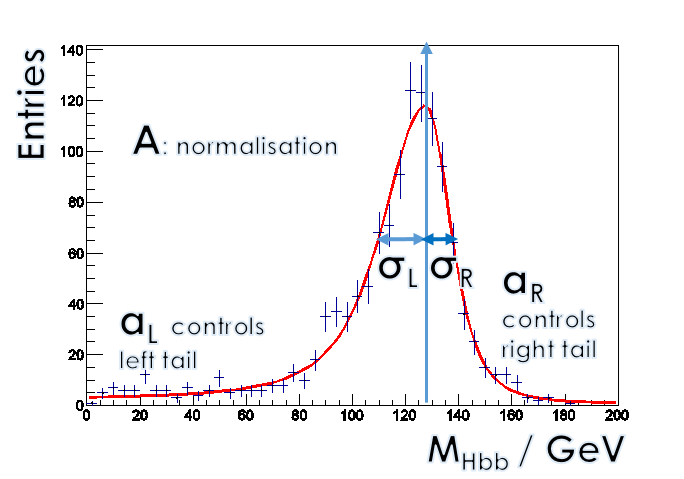
\includegraphics[width=\largefigwidth]{doubleHiggs/MCmassFit}
\caption[Example MC mass fit for double higgs analysis]%
   {A typical example of MC mass fit of $m_{\Hbb}$ for double higgs analysis. Red line indicates the best fit. Vertical arrow indicates the fitted peak position.}
   \label{fig:doubleHiggsFitMCMass}
\end{figure}

For \rootS{1.4}, shown in \Figure{fig:doubleHiggs1.4TeVMassFit}, \normalPFO with $R = 0.7$ give a good fitted mass for \HWW and \PW. The mass is slightly too low for the \Hbb. \Figure{fig:doubleHiggs1.4TeVSigmaFit} shows the combined relative fitted width for the \Hbb, \HWW and \PW. \NormalPFO with $R = 0.7$ gives an almost optimal relative width for \Hbb, while achieving a good balance for \HWW and \PW. Therefore, \normalPFO with $R = 0.7$ is chosen to be the optimal jet reconstruction parameters.

\begin{figure}[!tbp]
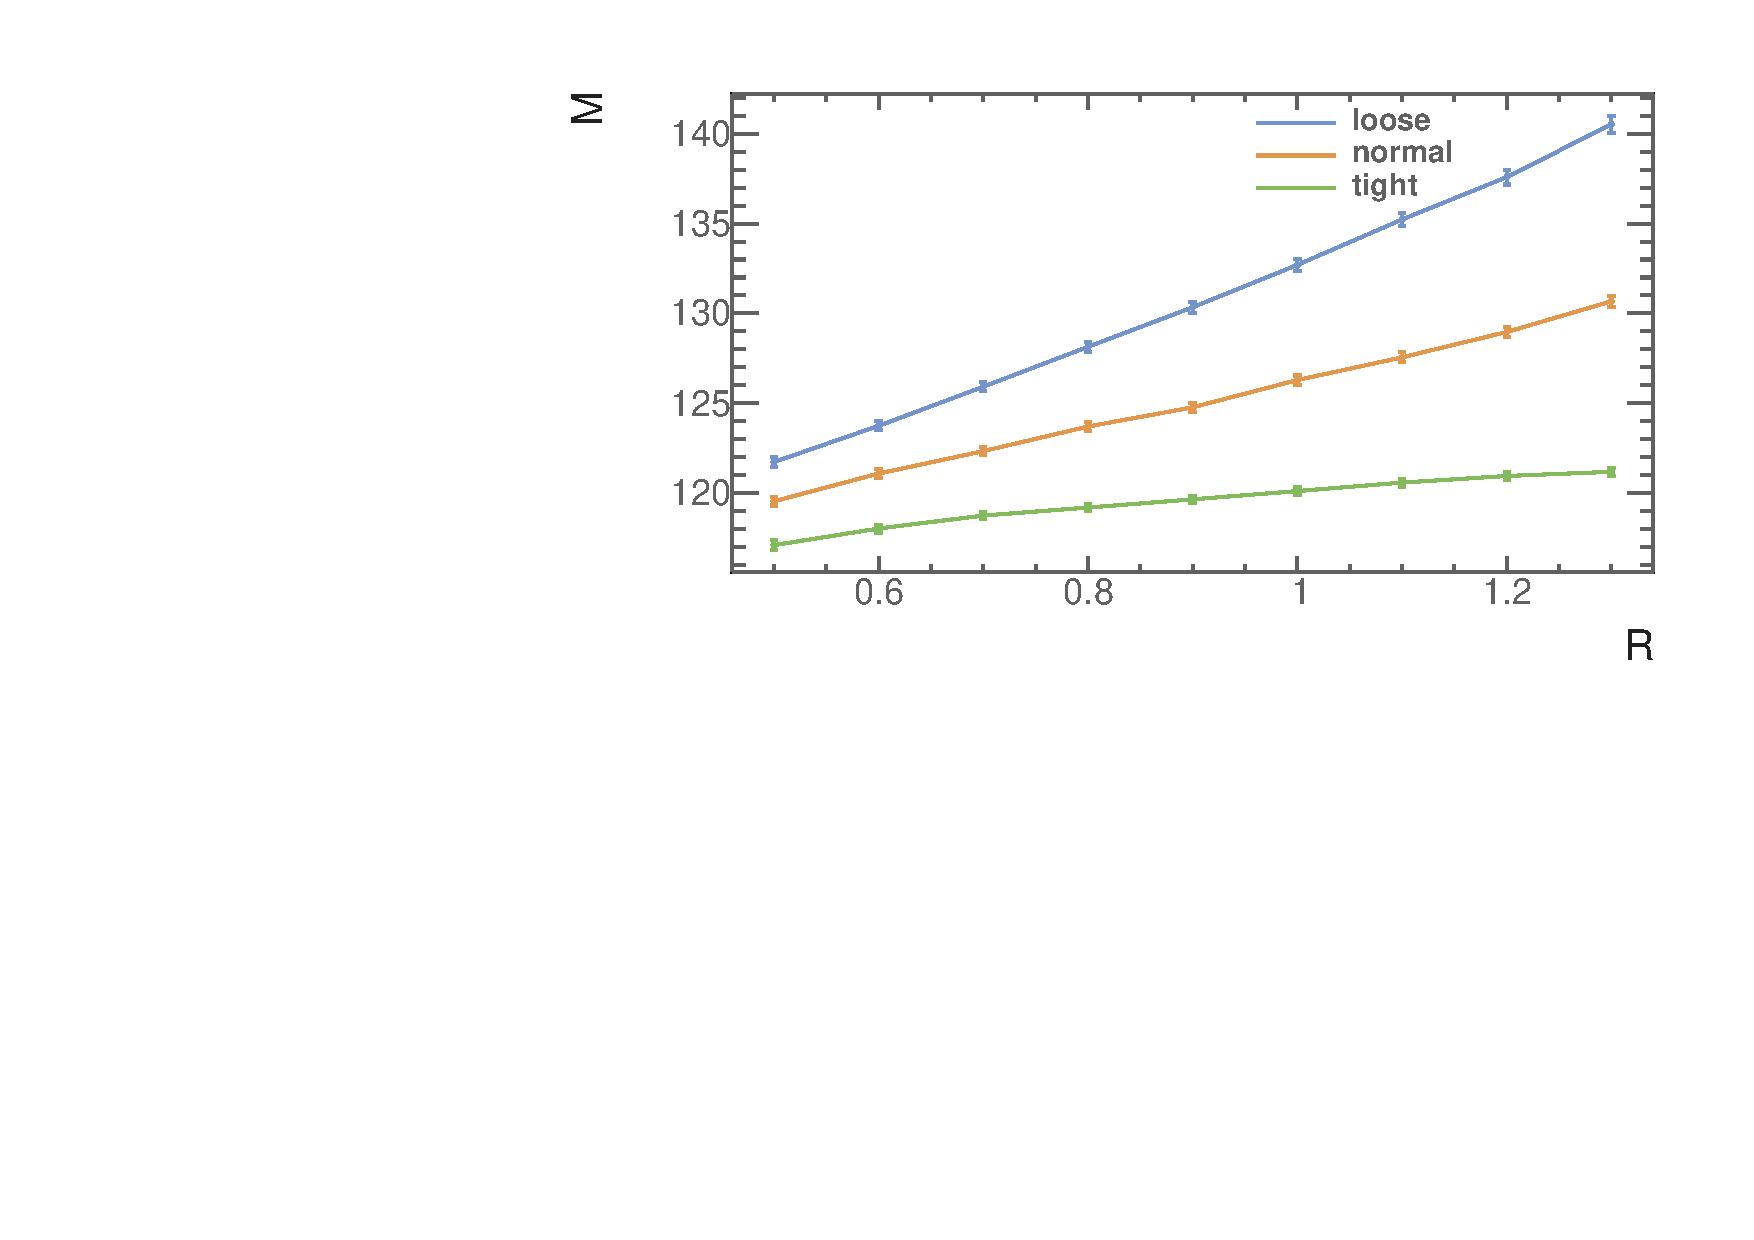
\includegraphics[width=\largefigwidth]{{{doubleHiggs/ILD_1.4TeV_Higgs1_M_R}}} \\
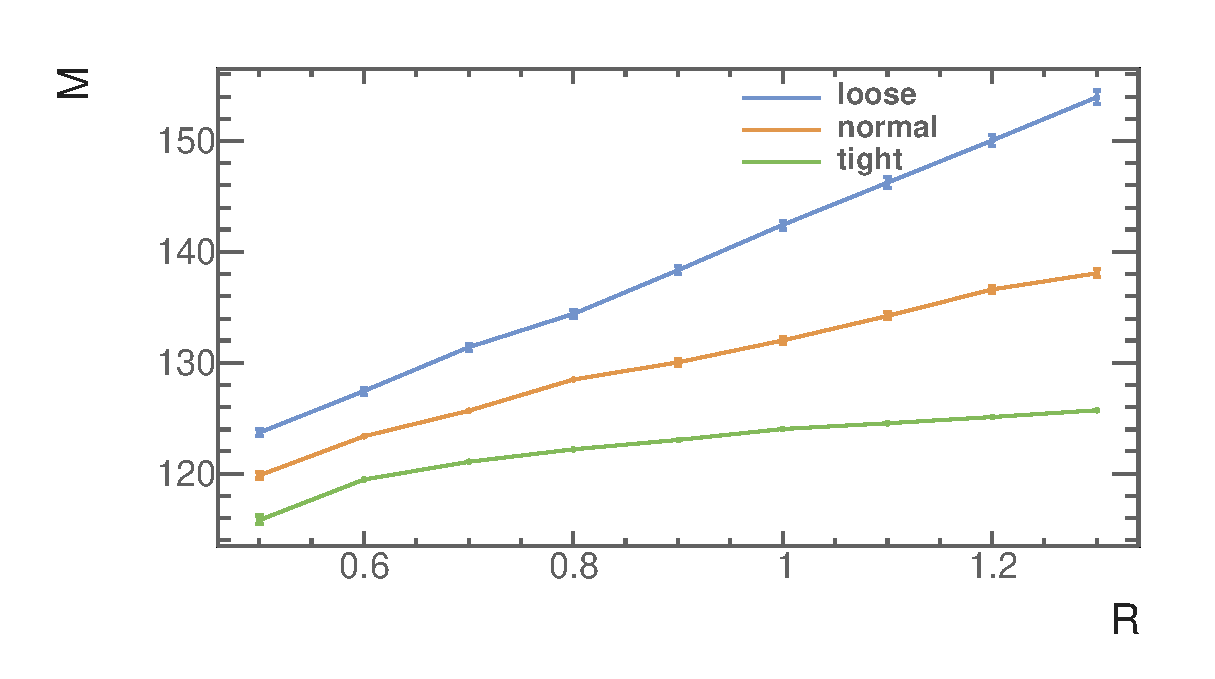
\includegraphics[width=\largefigwidth]{{{doubleHiggs/ILD_1.4TeV_Higgs2_M_R}}} \\
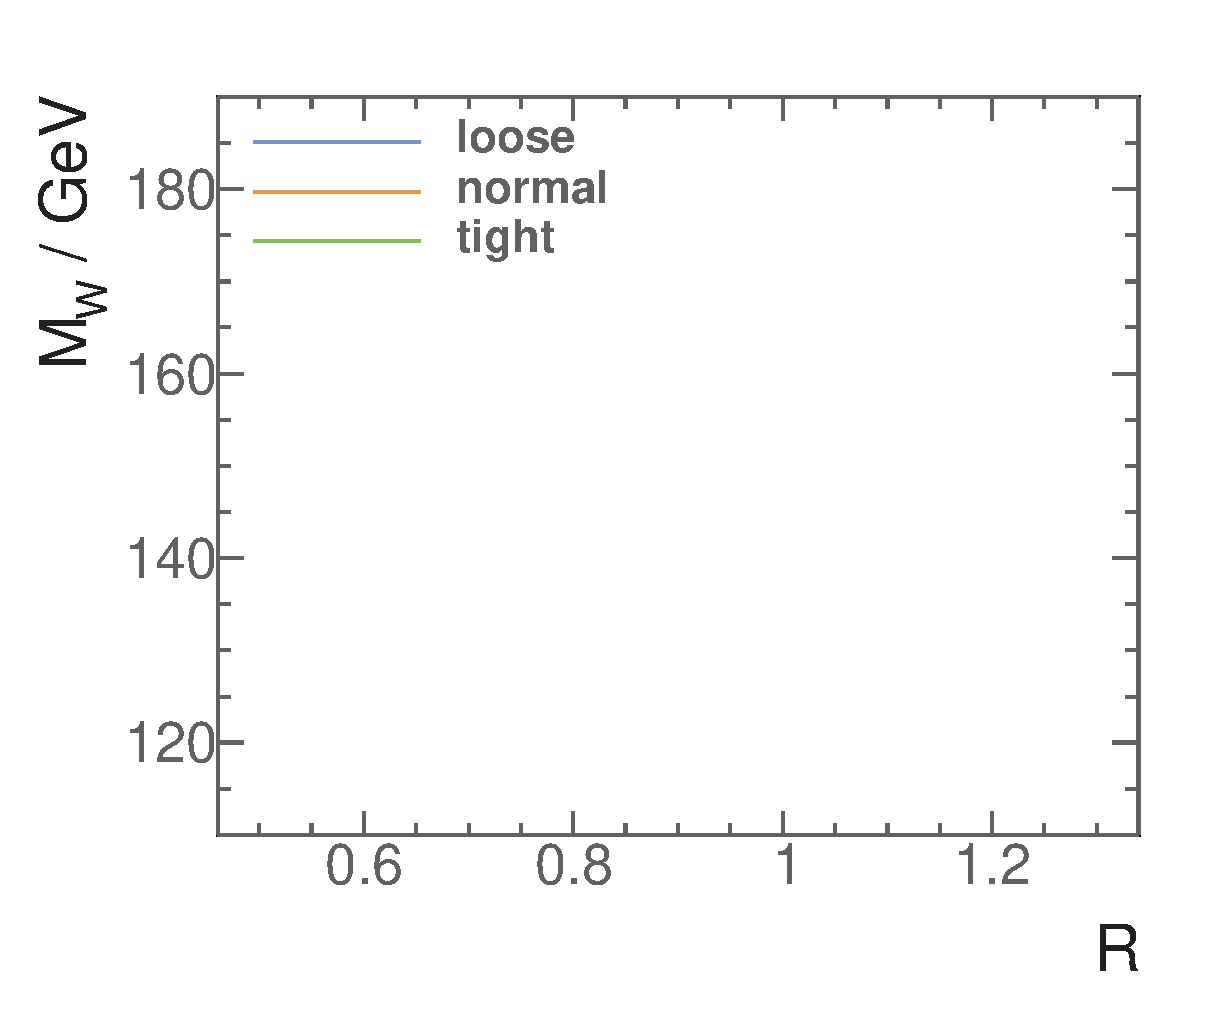
\includegraphics[width=\largefigwidth]{{{doubleHiggs/ILD_1.4TeV_W_M_R}}} \\
\caption[Fitted mass of \Hbb, \HWW and \PW for \rootS{1.4}]%
   {Fitted mass and error of \Hbb, \HWW and \PW for \rootS{1.4}, for loose, normal and tight selected PFO against $R$ parameter.}
   \label{fig:doubleHiggs1.4TeVMassFit}
\end{figure}

\begin{figure}[!tbp]
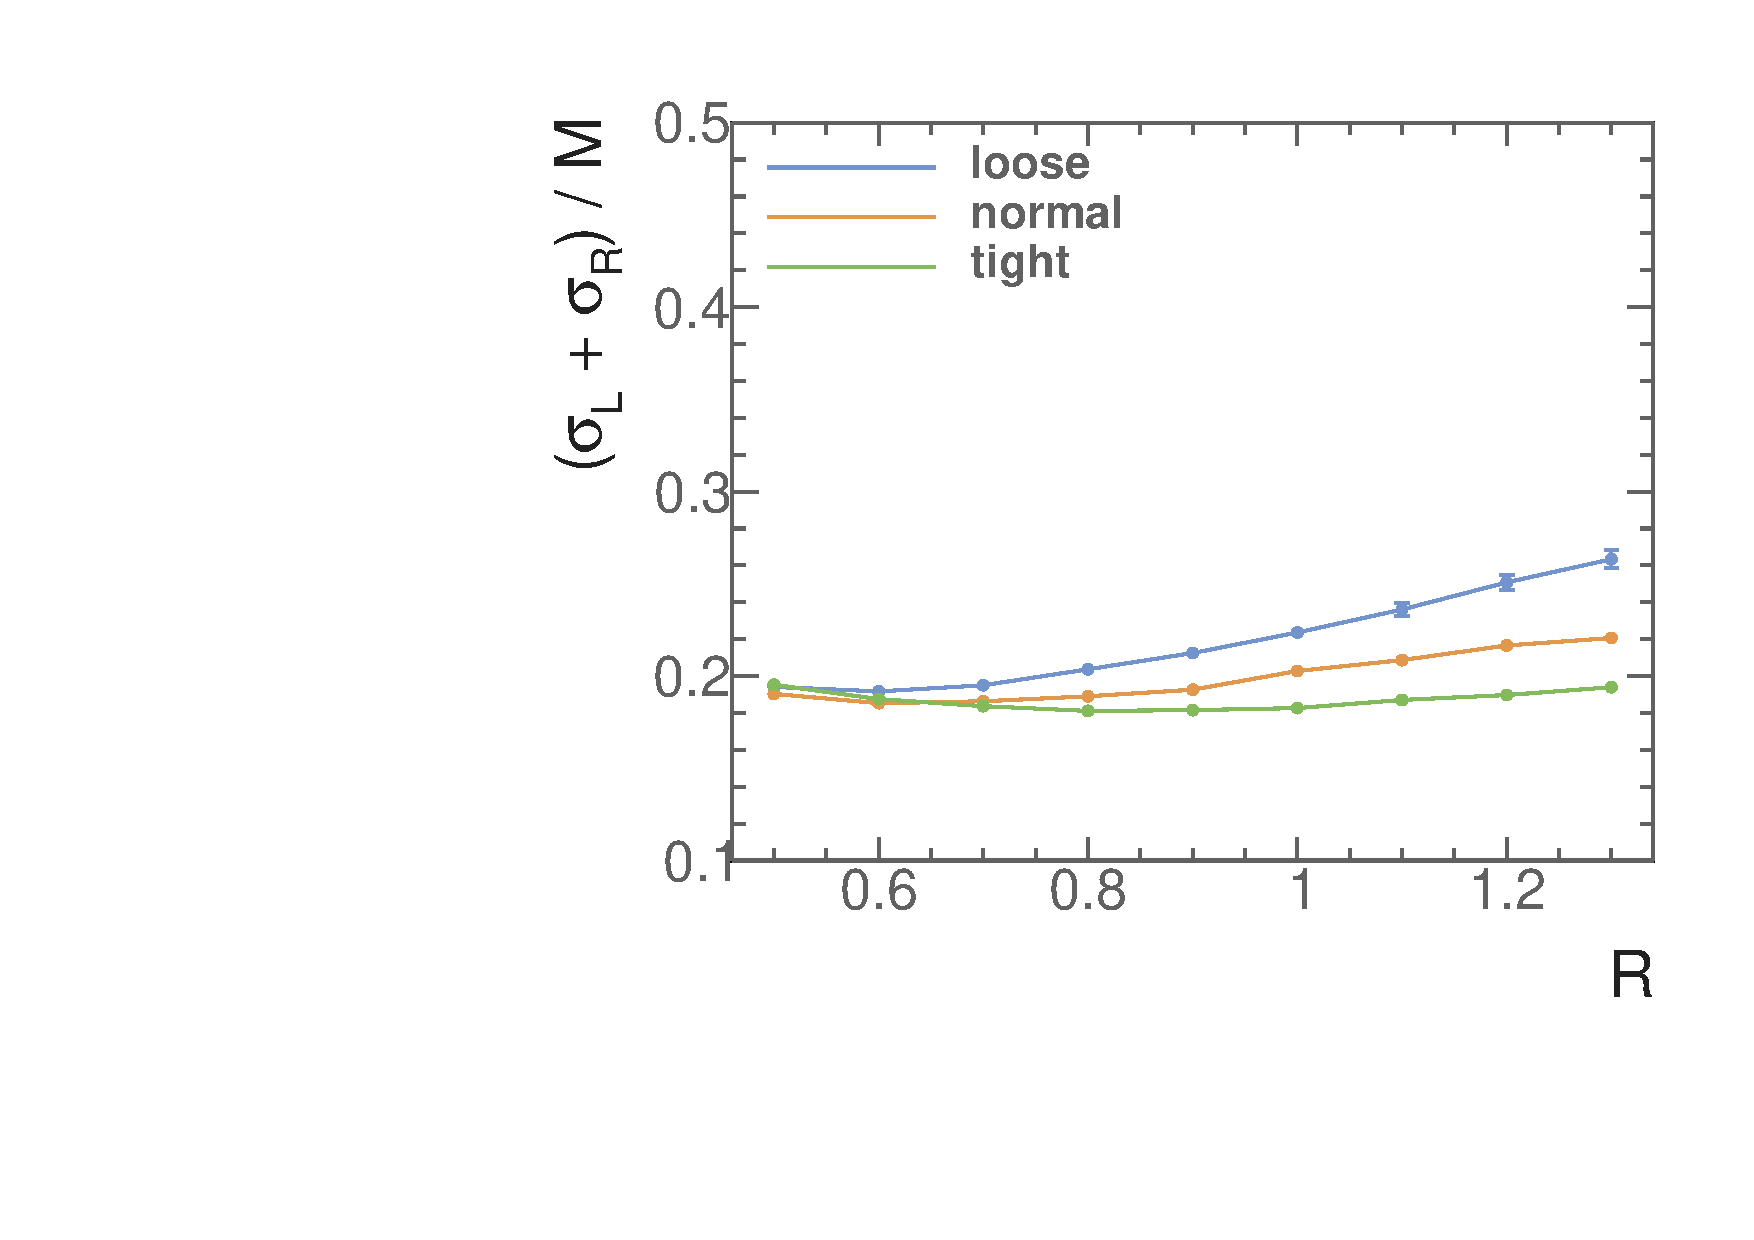
\includegraphics[width=\largefigwidth]{{{doubleHiggs/ILD_1.4TeV_Higgs1_SigmaL_add_SigmaR_divide_M_R}}} \\
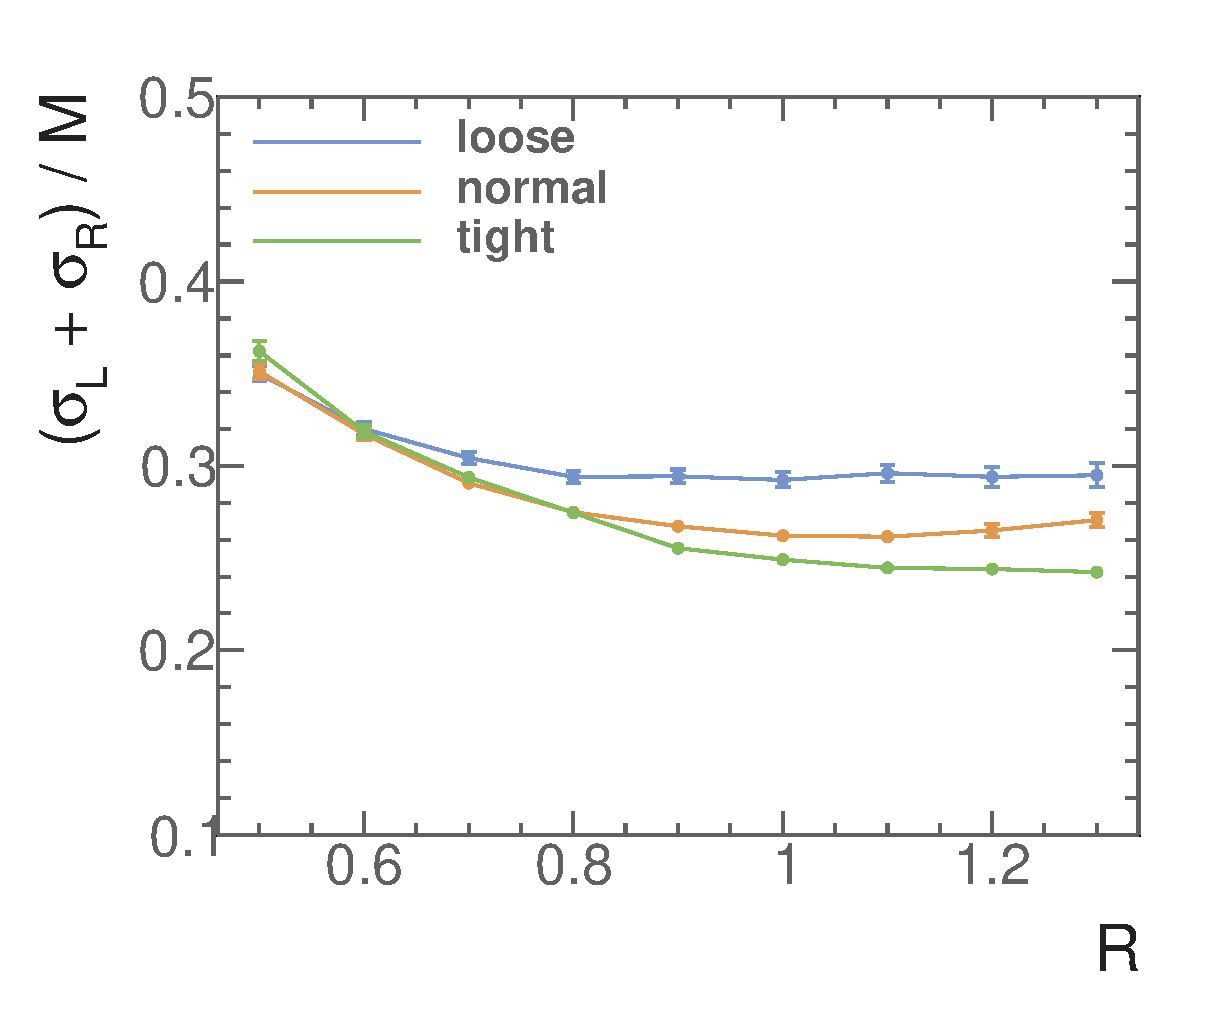
\includegraphics[width=\largefigwidth]{{{doubleHiggs/ILD_1.4TeV_Higgs2_SigmaL_add_SigmaR_divide_M_R}}} \\
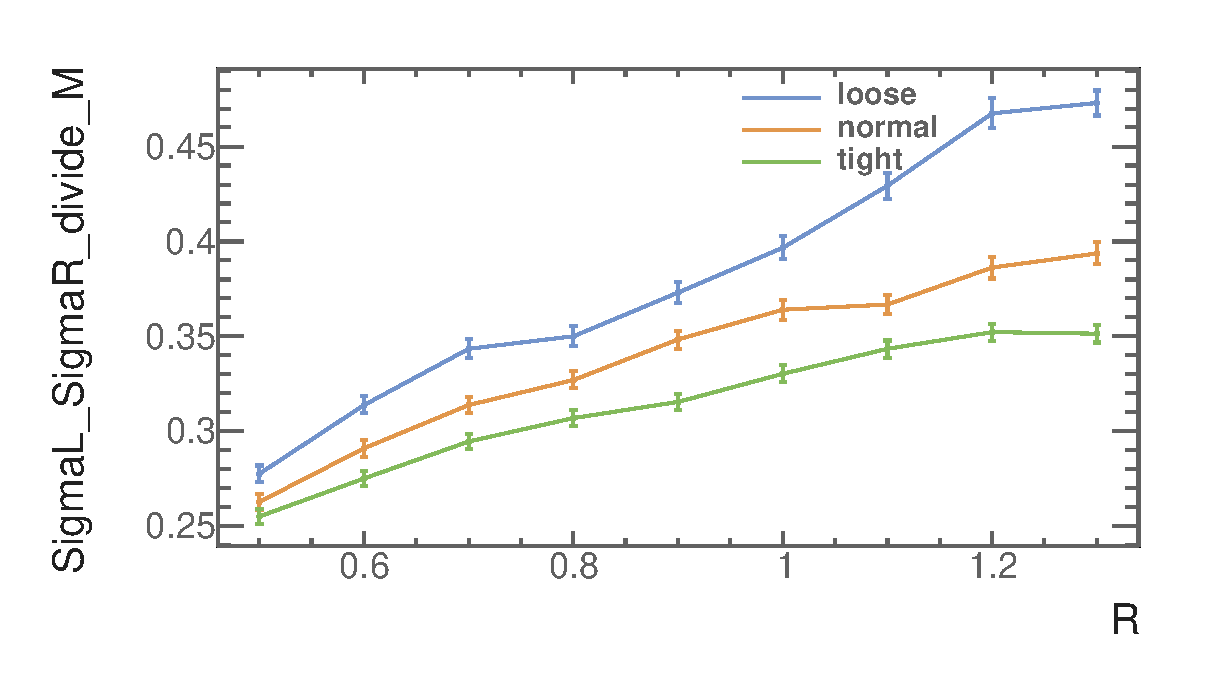
\includegraphics[width=\largefigwidth]{{{doubleHiggs/ILD_1.4TeV_W_SigmaL_add_SigmaR_divide_M_R}}} \\
\caption[Fitted width of \Hbb, \HWW and \PW for \rootS{1.4}]%
   {Fitted combined width and error of \Hbb, \HWW and \PW for \rootS{1.4}, for loose, normal and tight selected PFO against $R$ parameter.}
   \label{fig:doubleHiggs1.4TeVSigmaFit}
\end{figure}


For \rootS{3}, the choice is a bit more complicated. Shown in \Figure{fig:doubleHiggs3TeVMassFit}, fitted mass for \Hbb favours \normalPFO with $R = 0.8$. Fitted mass for \HWW favours \tightPFO with $R = 0.9$. Fitted mass for \PW favours \tightPFO with $R = 0.8$. Looking at the combined relative fitted width for the \Hbb, \HWW and \PW, shown in \Figure{fig:doubleHiggs3TeVSigmaFit}, \normalPFO gives a larger width than \tightPFO. Within \tightPFO, small $R$ values provide a shaper width for \HWW and \Hbb, but a broader width for \PW. Therefore, \tightPFO with $R = 0.7$ and $R = 1$ are both chosen for parallel analysis.

Later it was shown that \tightPFO with $R = 0.7$ gives a better signal significance. Therefore the optimal choice of jet reconstruction for \rootS{3} is \tightPFO with $R = 0.7$.

\begin{figure}[!tbp]
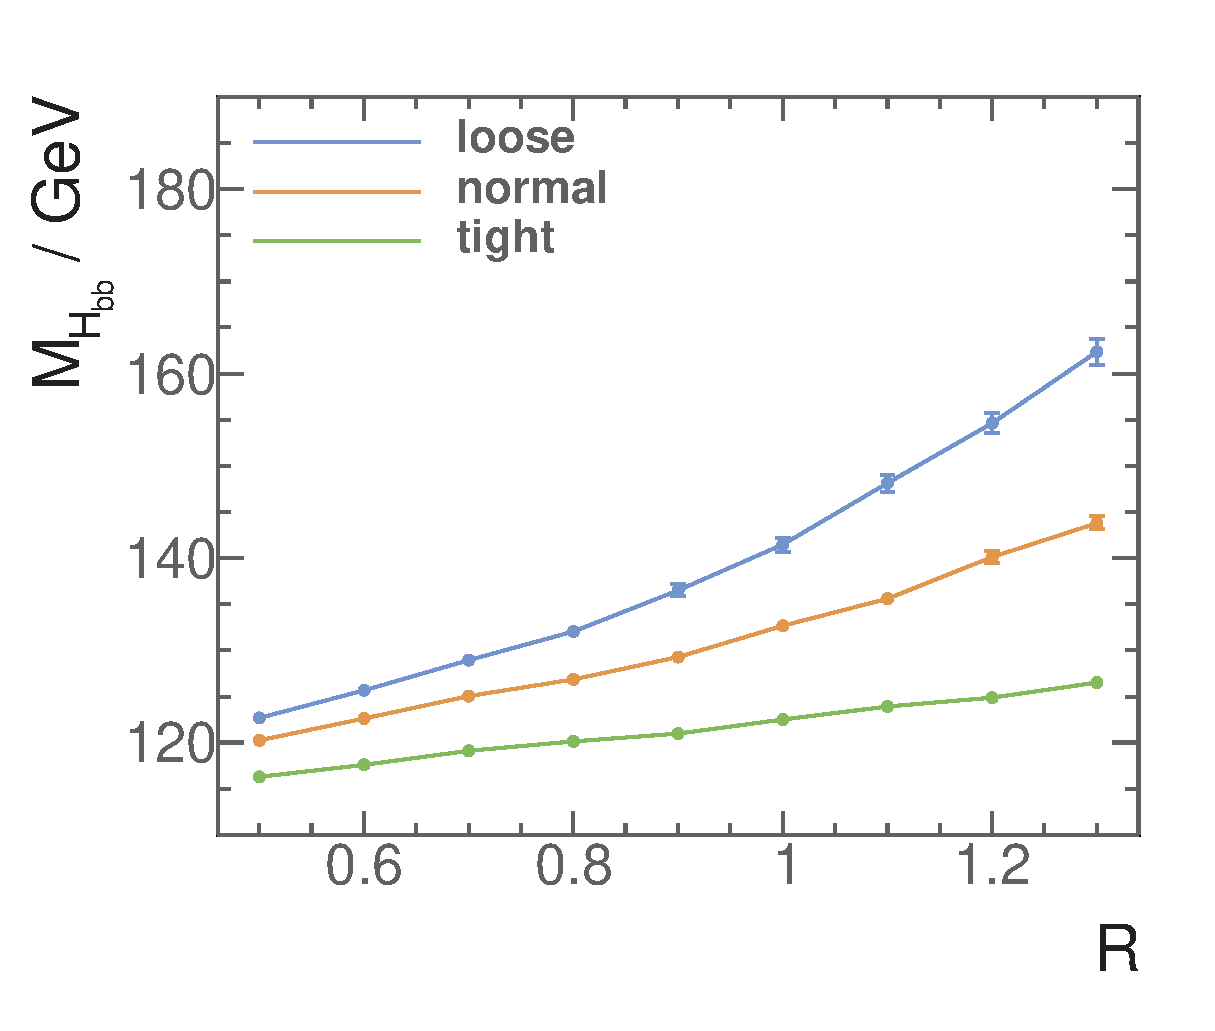
\includegraphics[width=\largefigwidth]{{{doubleHiggs/ILD_3TeV_Higgs1_M_R}}} \\
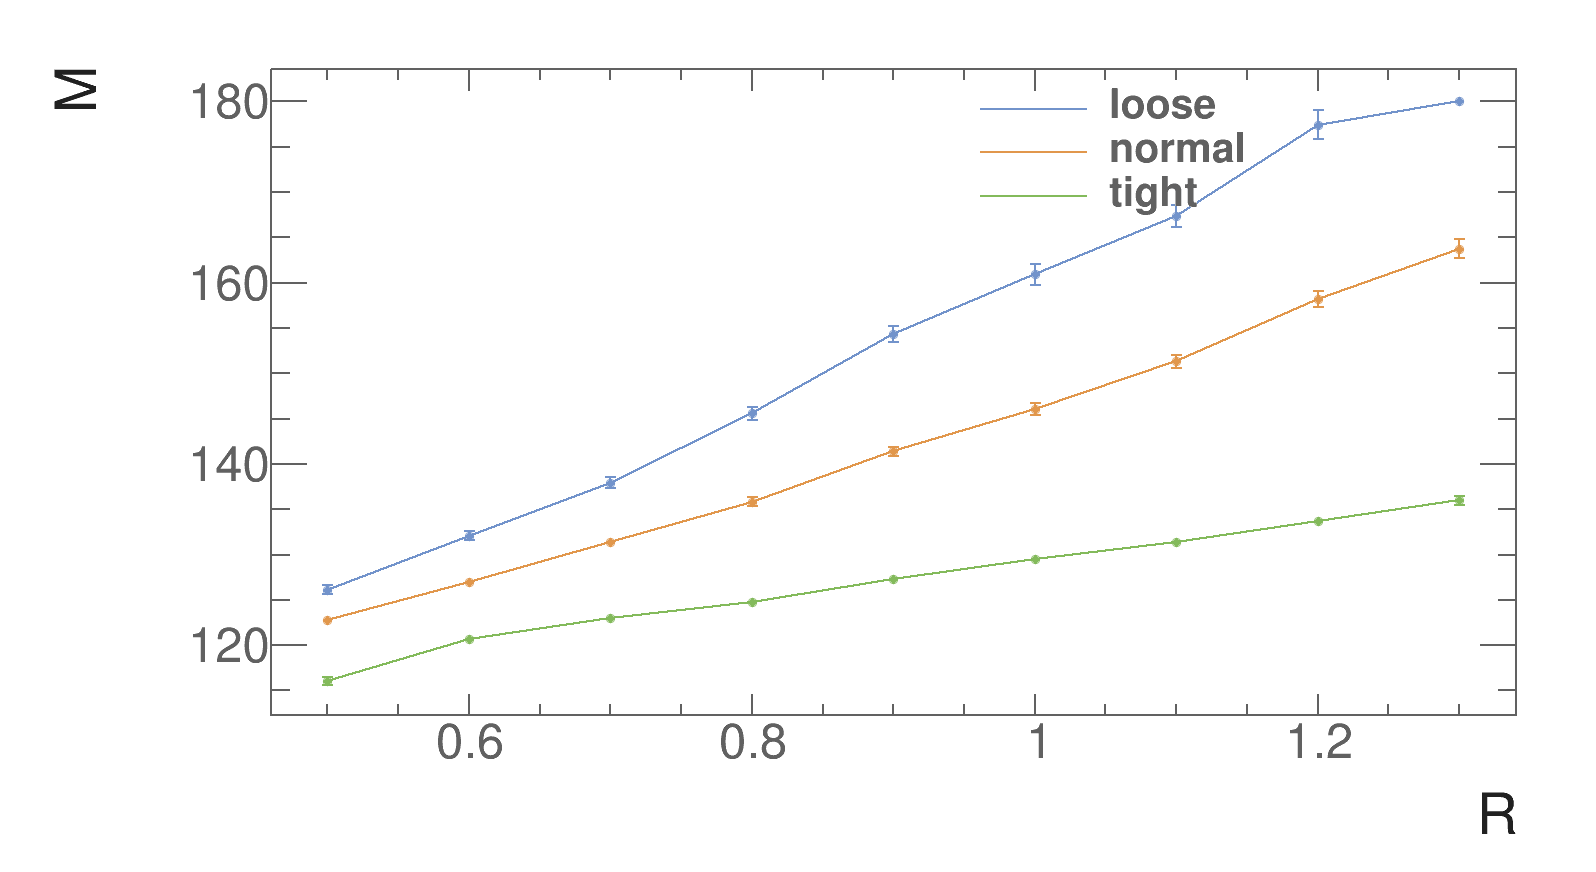
\includegraphics[width=\largefigwidth]{{{doubleHiggs/ILD_3TeV_Higgs2_M_R}}} \\
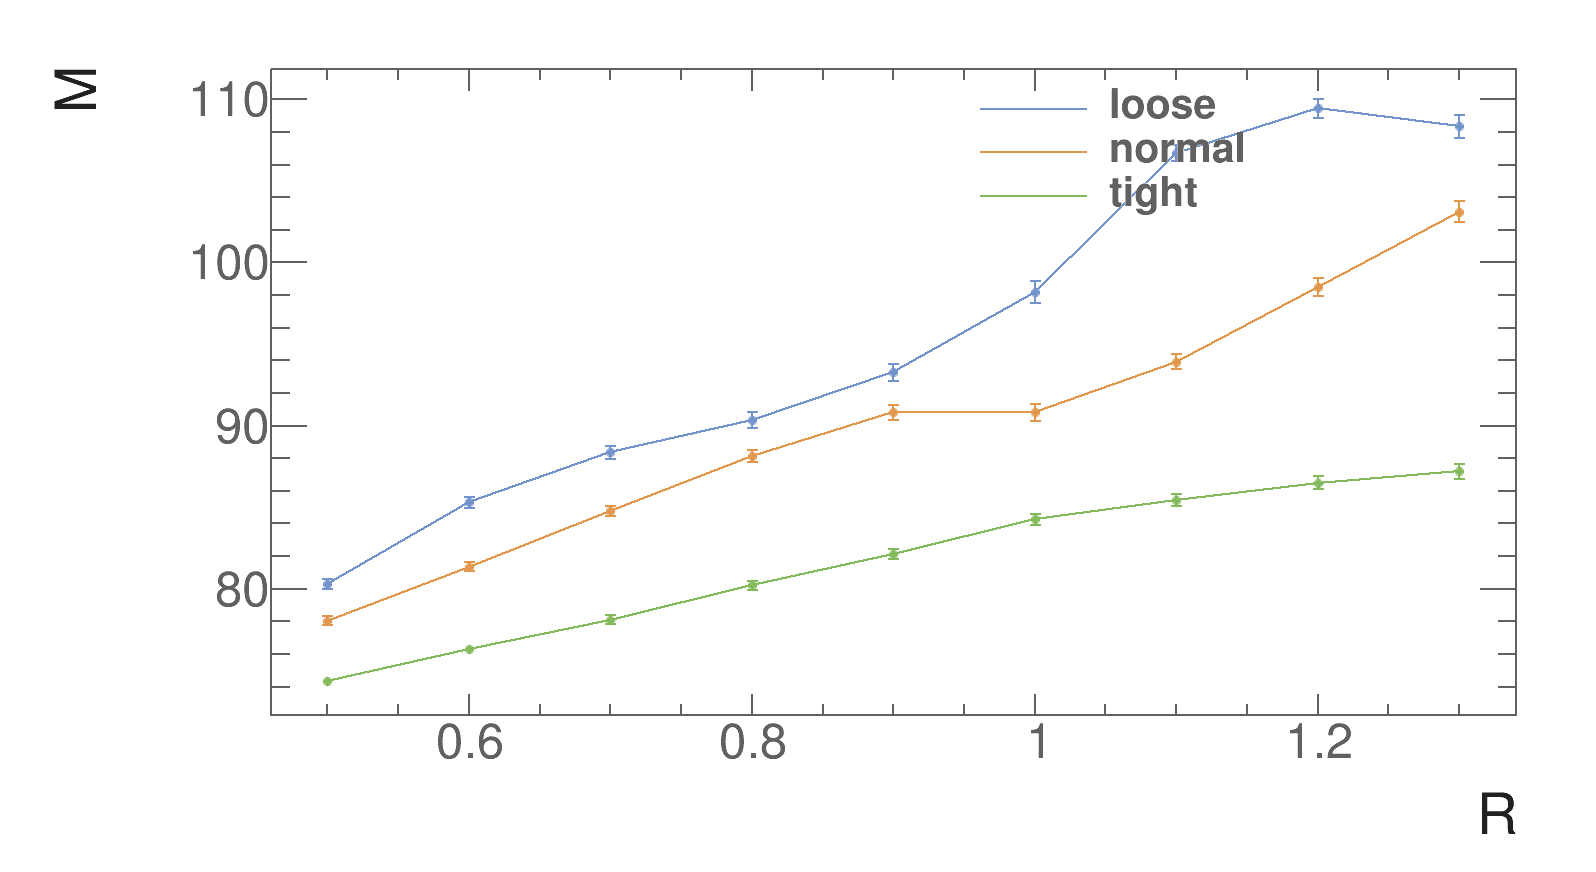
\includegraphics[width=\largefigwidth]{{{doubleHiggs/ILD_3TeV_W_M_R}}} \\
\caption[Fitted mass of \Hbb, \HWW and \PW for \rootS{3}]%
   {Fitted mass and error of \Hbb, \HWW and \PW for \rootS{3}, for loose, normal and tight selected PFO against $R$ parameter.}
   \label{fig:doubleHiggs3TeVMassFit}
\end{figure}

\begin{figure}[!tbp]
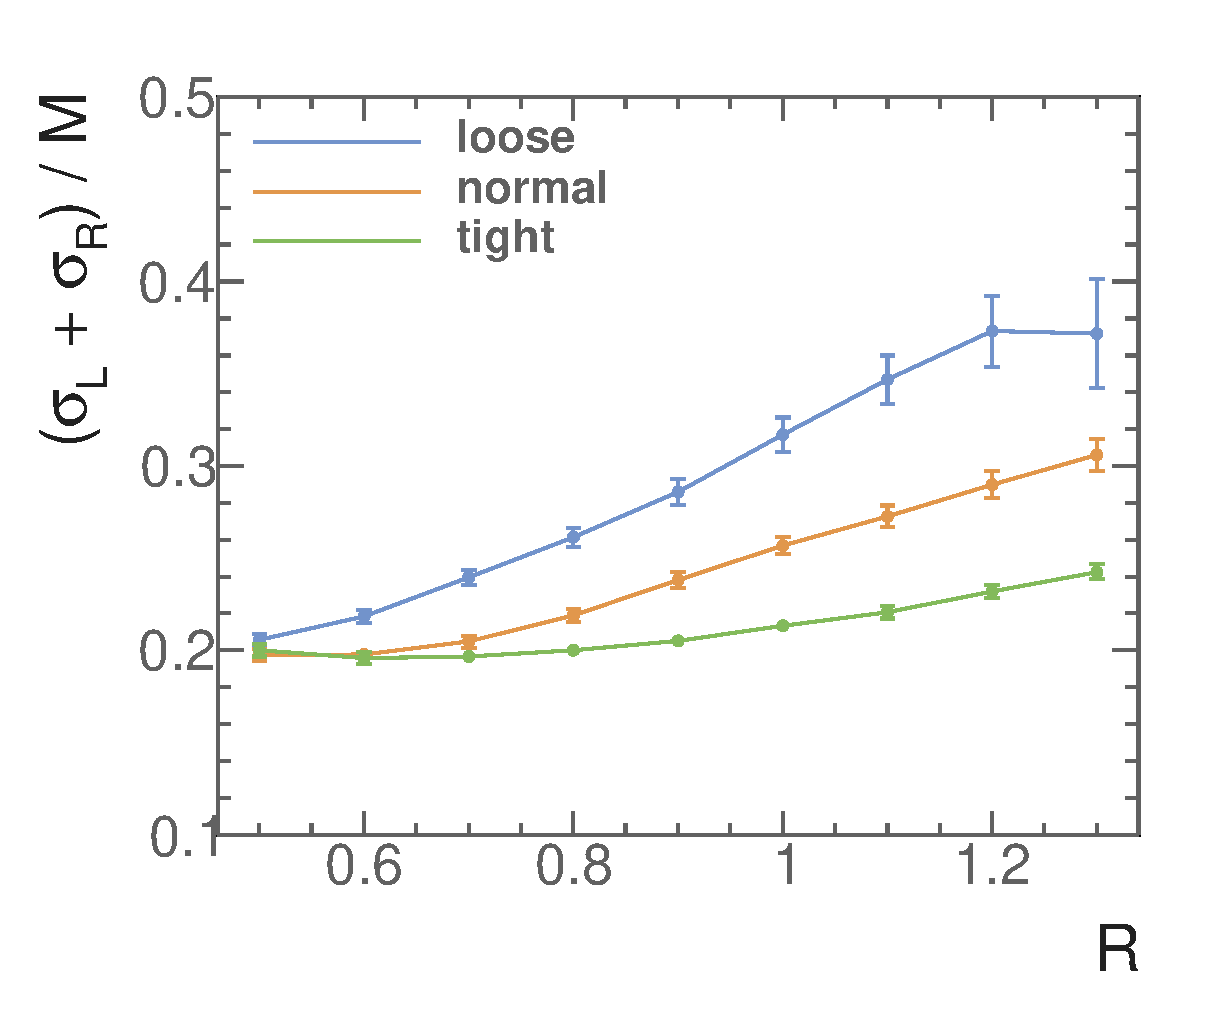
\includegraphics[width=\largefigwidth]{{{doubleHiggs/ILD_3TeV_Higgs1_SigmaL_add_SigmaR_divide_M_R}}} \\
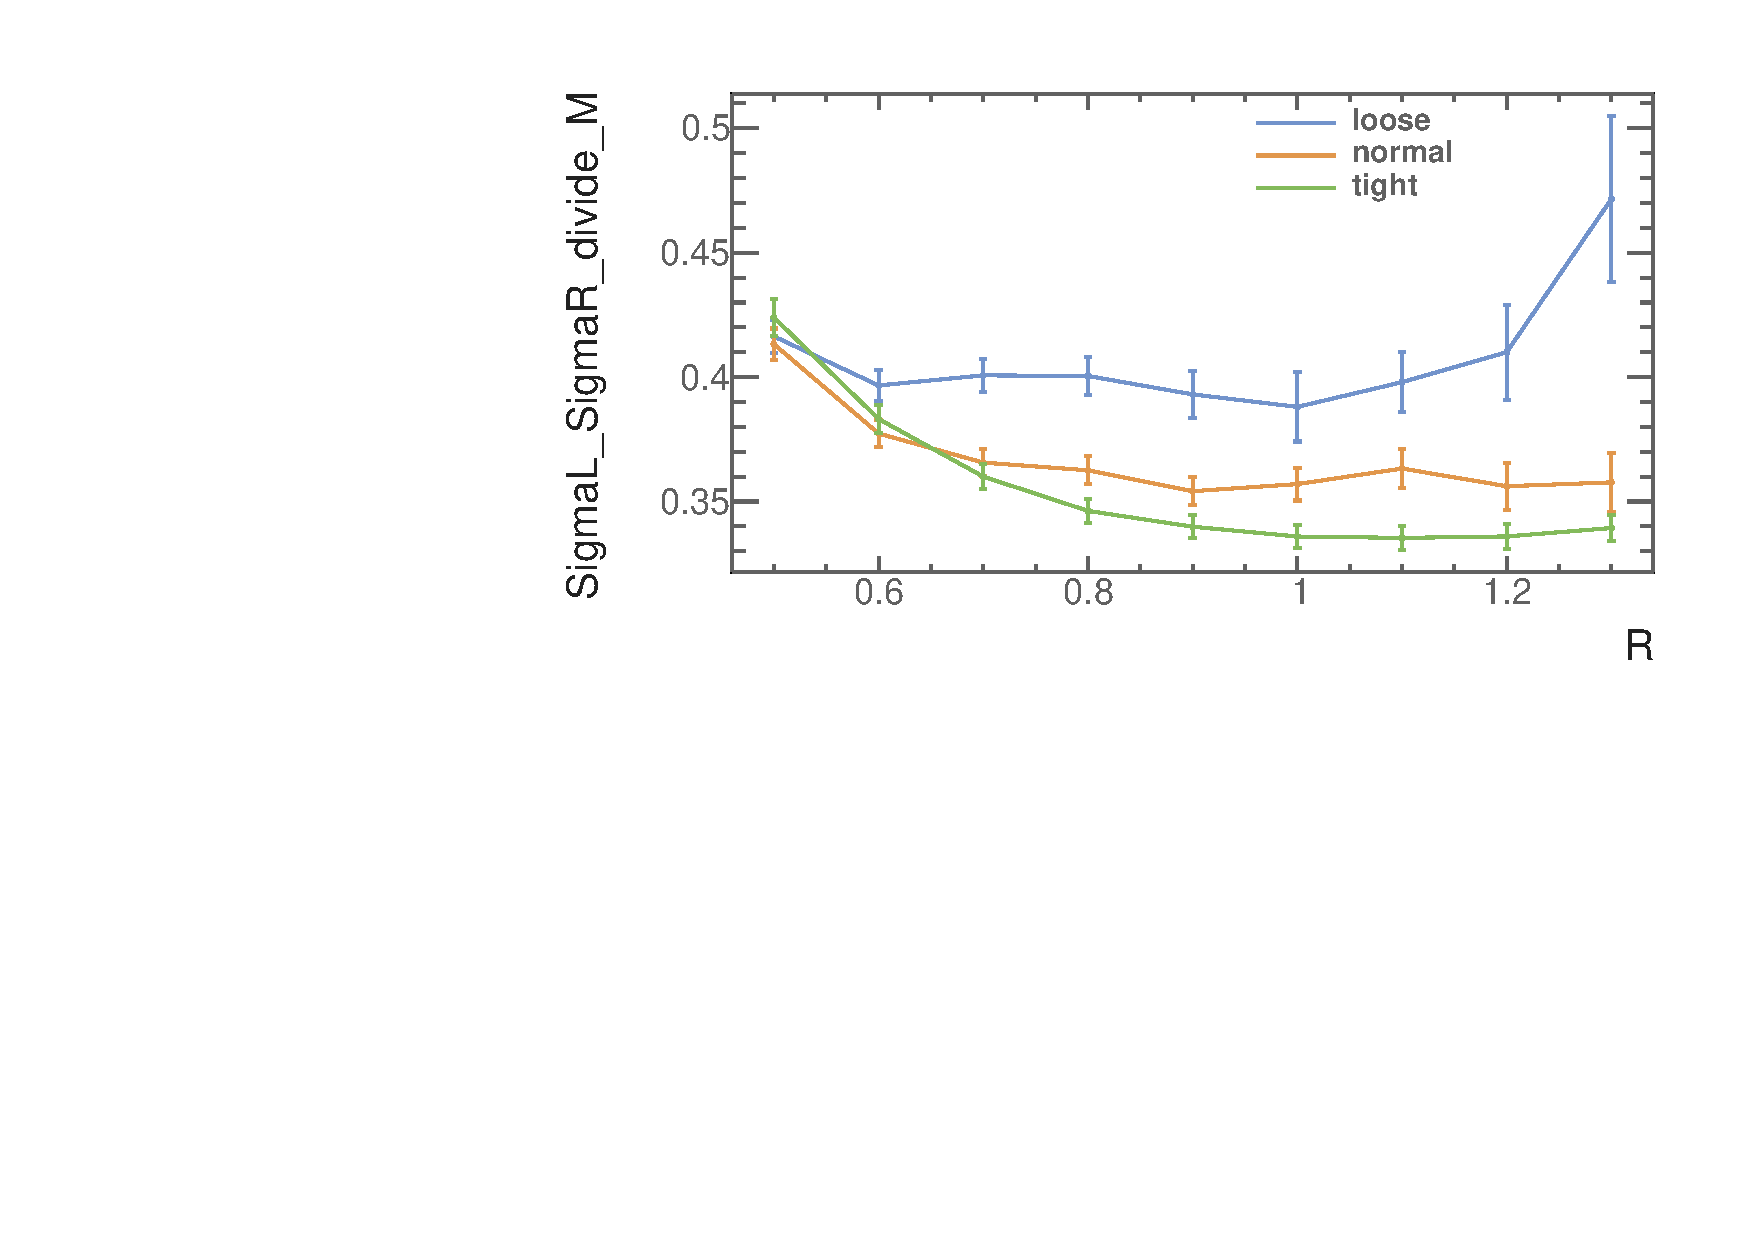
\includegraphics[width=\largefigwidth]{{{doubleHiggs/ILD_3TeV_Higgs2_SigmaL_add_SigmaR_divide_M_R}}} \\
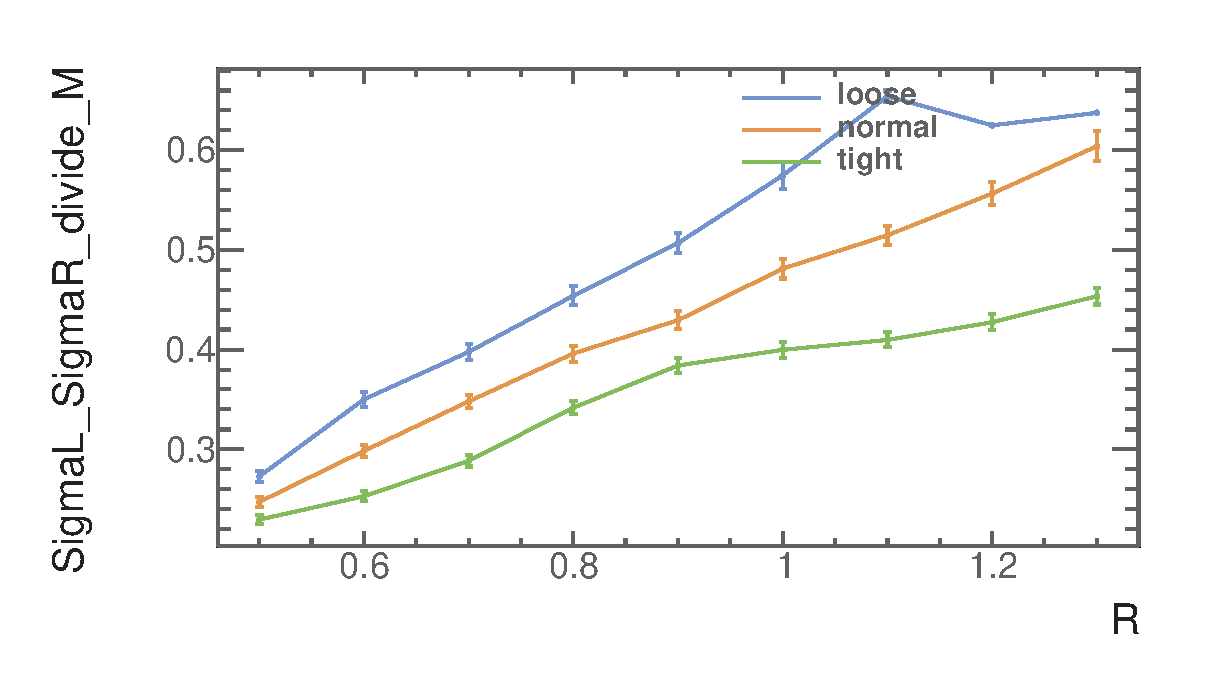
\includegraphics[width=\largefigwidth]{{{doubleHiggs/ILD_3TeV_W_SigmaL_add_SigmaR_divide_M_R}}} \\
\caption[Fitted width of \Hbb, \HWW and \PW for \rootS{3}]%
   {Fitted combined width and error of \Hbb, \HWW and \PW for \rootS{3}, for loose, normal and tight selected PFO against $R$ parameter.}
   \label{fig:doubleHiggs3TeVSigmaFit}
\end{figure}

\subsection{Jet flavour tagging} 

Two b-jets out of six jets in \HepProcess final states are identified with flavour tagging processors. The processor calculates a set of discriminatively variables for a jet. After training the MVA, the MVA is applied to jets to produce a likelihood for b-jet and c-jet. For details see \Section{}.

The existing LCFIPlus processor in Marlin package is used. The training sample of the flavour tagging processor is \HepProcess{\Pem \Pep \to \PZ \Pnu \APnu}, where \PZ decays to \HepProcess{\qlight\Aqlight}, \HepProcess{\Pbottom\APbottom}, or \HepProcess{\Pcharm\APcharm} at \rootS{1.4} and \rootS{3}, because they have similar event topology as the signal, and they have only two jets in the final state.

The selection efficiency of b-jets and c-jets with trainning samples are shown in \Figure{}. Flavour tagging performs better at low energy. Because at high energy, particles at more collimated and more difficult to separate.


\begin{figure}[!tbp]
  \begin{subfigure}[b]{0.45\textwidth}
    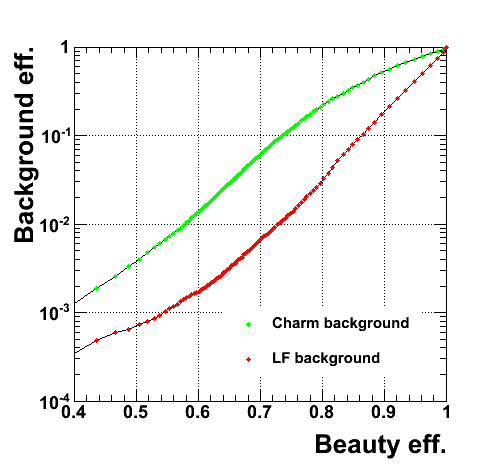
\includegraphics[width=\textwidth]{{{doubleHiggs/eval-lcfiweights_R0_7_2jets-test}}}
    \caption{\rootS{1.4}}
    \label{fig:doubleHiggs1.4Btag}
  \end{subfigure}
  \hfill
  \begin{subfigure}[b]{0.45\textwidth}
    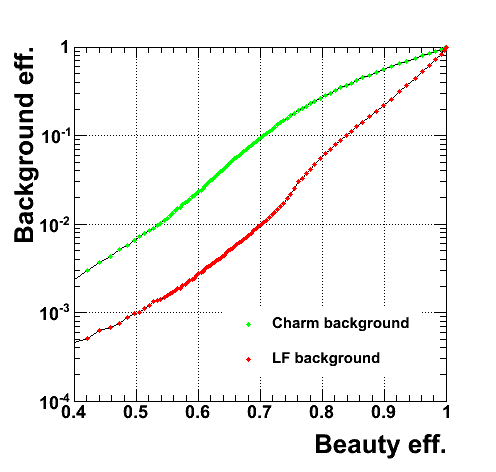
\includegraphics[width=\textwidth]{{{doubleHiggs/eval-lcfiweights_tR0_7_3000_2jets-test}}} 
    \caption{\rootS{3}}
    \label{fig:doubleHiggs3Btag}
  \end{subfigure}
    \caption[Performance of b-jet tagging with trainning samples]%
   {Performance of b-jet tagging with trainning samples}
   \label{fig:doubleHiggsBtag}
\end{figure}

\subsection{Jet pairing}

The jet pairing was performed by seaking combination of jets that are compatible with signal \eeToHHbbWW. 

The actual pairing is done via a minimisation
\begin{equation}
	\chi^2 = \left(\frac{m_{ij}-m_{\Hbb}}{\sigma_{\Hbb}^*}\right)^2 + \left(\frac{m_{klmn}-m_{\HWW}}{\sigma_{\HWW}^*}\right)^2  + \left(\frac{m_{kl}-m_{\PW}}{\sigma_{\PW}^*}\right)^2,
%\label{eqn:eq_chi2_HHWWbb}
\end{equation}
where, $m_{\Hbb}$ and 


\begin{comment}
One of the key points in the analysis is the mass reconstruction. In particular, to associate the correct jets to each Higgs boson.

The \HHWWbb hadronic channel, with its 6 jets, is the most complex case.
All possible combinatorics are tested and the one that minimises the following criteria is chosen:
\begin{equation}
	\chi^2 = \left(\frac{m_{ij}-\mh}{\sigma_{H_{bb}}}\right)^2 + \left(\frac{m_{klmn}-\mh}{\sigma_{H_{WW}}}\right)^2  + \left(\frac{m_{op}-m_{W}}{\sigma_{W}}\right)^2,
\label{eq_chi2_HHWWbb}
\end{equation}
where the Higgs mass, \mh, is assumed of \SI{126}{GeV} and the $W$ mass, $m_W$, is assumed of \SI{80.385}{GeV}. The expected resolution for each mass distribution, $\sigma_{H_{bb}}$, $\sigma_{H_{WW}}$ and $\sigma_{W}$, is extracted from the following function by assigning to each objects the right jet pair. The values so obtained are: $\sigma_{H_{bb}} = ...$, $\sigma_{H_{WW}} = ...$ and $\sigma_{W} = ...$ .

% TODO add the fitting function
\end{comment}